%************************************************
\chapter{Causally Reflective Procedural Tracing}
\label{chapter:causally_reflective_procedural_tracing}
%************************************************

The parallel fiber virtual machines create, mutate, and read from
memory as they execute sequences of bytecodes.  At any given point,
the SALS memory system is static.  The current execution state of
every fiber is represented in the global environment.  In order for
SALS to be fully reflective on all of the procedural effects of any
given fiber, I introduce a technique that I call \emph{causal
  reflective tracing}.  Causal reflective tracing is simply a way of
defining variables that are specific to each fiber that can be used to
control the low-level memory access, mutation, and creation functions.
This allows one fiber within SALS to subscribe to the procedural trace
events of another fiber without receiving procedural trace events of
its own execution, which would lead to an infinite regress, halting
the system.  Further, because SALS is inherently a parallel processing
system, a given fiber will often start a number of child fibers that
handle part of the processing for the parent fiber.  When a new fiber
is created, the child fiber inherits the causal variable bindings of
its parent fiber, enabling the same procedural tracing options for the
child as well.  So, causal reflective tracing is one of the basic
tools for keeping track of which pieces of memory were created,
mutated, or read by which other fibers.

Creating procedural trace events for the execution of a given fiber
slows the fiber down by a constant factor.  This is an important point
to consider when evaluating the theoretical time complexity of
concurrent procedurally reflective control algorithms.

\section{Semantic Memory Focuses Reflective Tracing}

While causal reflective tracing focuses the procedural event tracing
to memory interactions of specific fibers, this still results in
millions of events to consider every real-time second of execution.
In order to further focus the reflective tracing focus to specific
objects within the SALS memory system, specific pieces of memory can
be marked as \emph{semantic memory}.  Semantic memory objects are
created, mutated, and accessed in roughly the same way as all of the
frame-based objects in the SALS memory system.  Semantic memory
objects provide event streams that can be subscribed to by a number of
different parallel listeners in different fibers.  The following code
example shows how frame-based objects with default slot values and
constructors are used to define a {\tt Planning-Machine} type object:
\begin{equation*}
\begin{array}{l}
\text{\tt [deframe Planning-Machine [layer} \\
\text{\tt ~~~~~~~~~~~~~~~~~~~~~~~~~~~~[focus ~~~~~~~~~nil]} \\
\text{\tt ~~~~~~~~~~~~~~~~~~~~~~~~~~~~[execute ~~~~~~~nil]} \\
\text{\tt ~~~~~~~~~~~~~~~~~~~~~~~~~~~~[register-a ~~~~nil]} \\
\text{\tt ~~~~~~~~~~~~~~~~~~~~~~~~~~~~[register-b ~~~~nil]} \\
\text{\tt ~~~~~~~~~~~~~~~~~~~~~~~~~~~~[register-c ~~~~nil]} \\
\text{\tt ~~~~~~~~~~~~~~~~~~~~~~~~~~~~[positive-goals nil]} \\
\text{\tt ~~~~~~~~~~~~~~~~~~~~~~~~~~~~[negative-goals nil]]} \\
\text{\tt ~~[new [initial-layer]} \\
\text{\tt ~~~~[= layer initial-layer]} \\
\text{\tt ~~~~nil]]}
\end{array}
\end{equation*}
Once a frame-based object is defined, the ``{\tt new}'' operator is
used in order to create a new instance of the object type as in the
following example:
\begin{equation*}
\begin{array}{l}
\text{\tt [new Planning-Machine `Reflective-1]} \\
\end{array}
\end{equation*}

\section{Forgetful Event Streams}

By default, when there are no listeners to the procedural event
streams of a semantic frame-based object, no reflective events are
created, allowing the use of the object to run at full speed.  When a
listener subscribes to the procedural use of a specific semantic
memory object, events are added to ordered streams for the listening
subscribers.  In order to conserve memory resources, when multiple
parallel listeners are subscribed to a given event stream, only those
events that have not already been seen by all of the subscribers are
remembered.  Once all subscribers have processed an event, all events
before this event are forgotten.  This type of memory conserving event
stream is referred to as a \emph{forgetful event stream}.  In this way
semantic frames report the addition and removal of slot values to
reflective forgetful event stream subscribers.

\section{Semantic Knowledge-Bases}

Because it becomes awkward to subscribe to each an every frame-based
object that may be interesting to the reflective focus, semantic
frames that are created by specific fibers can be added to collections
of semantic frames that are called \emph{semantic knowledge-bases}.
Semantic knowledge-bases are good for organizing entire layers or
subsets of reflective layers that contain different types of semantic
frames.  Semantic knowledge-bases allow the same forgetful event
stream subscription services as semantic frames with the additional
capability of tracing the addition and removal of entire semantic
frames to and from the knowledge-base.

\section{Reflectively Reconstructed Semantic Knowledge-Bases}

Each parallel subscriber to the reflective procedural knowledge-base
events receives each event slightly after it occurs.  It often becomes
necessary to be able to refer to the historical state of the
knowledge-base under the reflective focus.  However, in order to not
slow down the primary procedure, the primary knowledge base must be
allowed to change during the time that it takes the reflective process
to process each event.  In this case, it becomes necessary to maintain
accurate reflective reconstructions of knowledge-bases that are
accurate at the reflective time of each reflective event that is
processed in parallel.  For example, in order to implement symbolic
perception, each slot value addition to the physical knowledge-base is
reflectively traced and the physical knowledge base is constructed as
a reflective copy that is accurate to the reflective time.  This
\emph{reflectively reconstructed semantic knowledge-base} is used to
perform a check of the immediate frame-based graph surroundings of the
change to see if one of the symbolic perceptions has become active or
inactive due to the change.

\section{Semantic Event Interval-Tree Knowledge-Bases}

While knowledge-base reconstructions are extremely fast to reference,
$O(1)$, they require a duplication of the memory requirements of the
focus knowledge base for every different point in time that is
required.  In order to allow efficient access of the state of
knowledge-bases at arbitrary points in the past, \emph{semantic event
  interval-tree knowledge-bases} are another type of representation
that is reflectively maintained without slowing down the procedure
under reflective focus.  A semantic event knowledge-base stores a type
of semantic frame that represents when a given semantic frame has a
specific slot value called a \emph{semantic event}.  A semantic event
is a semantic frame is an interval that spans a time from a beginning
time and an ending time, each of which may or may not be specified.
Semantic event knowledge-bases are reflectively traced and the
knowledge is always stored in two different representations, the basic
semantic event frames as well as a balanced interval tree that always
represents the current state of the semantic event knowledge-base.
The balanced interval tree allows accessing the state of the focus
knowledge-base in $O(log n)$ time, where $n$ is the number of events
stored in the semantic event knowledge base.  Although the time
complexity is not as efficient as the constant, $O(1)$, access time of
the reflectively reconstructed semantic knowledge-base, the semantic
event interval-tree knowledge base only requires $O(n)$ memory
complexity in order to allow access to the structure of the
knowledge-base at any point in the past, where $n$ is the number of
semantic events.

\section{Implemented Physical Knowledge}

{\mbox{\autoref{figure:implemented_physical_knowledge}}} shows the
implemented physical knowledge.
\begin{figure}
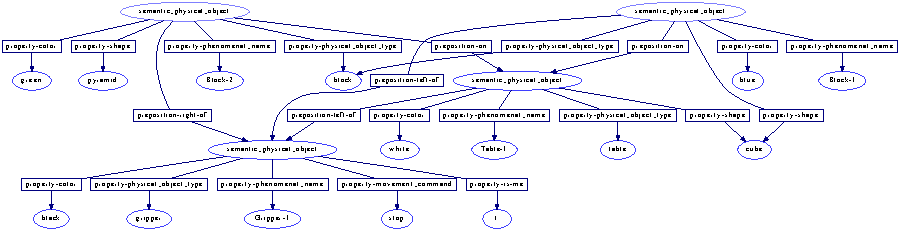
\includegraphics[width=10cm]{gfx/implemented_physical_knowledge}
\caption[The implemented physical knowledge.]{The implemented physical
  knowledge.}
\label{figure:implemented_physical_knowledge}
\end{figure}

\section{Implemented First-order Resource Activator}

{\mbox{\autoref{figure:implemented_first_order_resource_activator}}}
shows the implemented first-order resource activator.
\begin{figure}
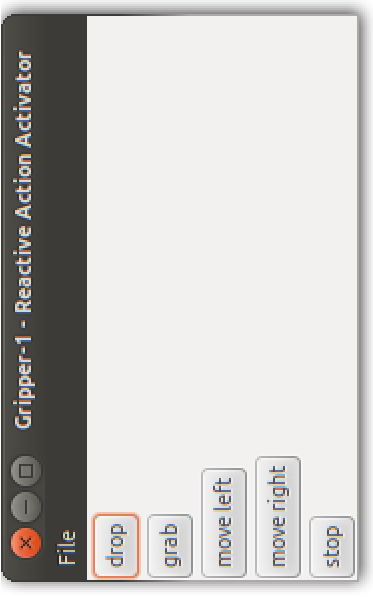
\includegraphics[width=10cm]{gfx/implemented_first_order_resource_activator}
\caption[The implemented first-order resource activator.]{The
  implemented first-order resource activator.}
\label{figure:implemented_first_order_resource_activator}
\end{figure}

